\documentclass[conference]{IEEEtran}
\IEEEoverridecommandlockouts
% The preceding line is only needed to identify funding in the first footnote. If that is unneeded, please comment it out.
\usepackage{cite}
\usepackage{amsmath,amssymb,amsfonts}
\usepackage{algorithmic}
\usepackage{graphicx}
\graphicspath{{./figures/}{IR}}
\usepackage{textcomp}
\usepackage{xcolor}
\usepackage{hyperref}
\def\BibTeX{{\rm B\kern-.05em{\sc i\kern-.025em b}\kern-.08em
    T\kern-.1667em\lower.7ex\hbox{E}\kern-.125emX}}
\bibliographystyle{IEEEtran}

\begin{document}

\title{Culinary Computation\\
{\footnotesize \textsuperscript{*}Data Analysis for Novel Recipe Generation}
\thanks{Portland State University Undergraduate Research Mentorship Program}
}

\author{\IEEEauthorblockN{1\textsuperscript{st} Nelson}
\IEEEauthorblockA{\textit{Computer Science} \\
\textit{Portland State University}\\
Portland, United States\\
ajn6@pdx.edu}
\and
\IEEEauthorblockN{2\textsuperscript{nd} Vassilevski}
\IEEEauthorblockA{\textit{Mathematics} \\
\textit{Portland State University}\\
Portland, United States\\
panayot@pdx.edu}
}

\maketitle

\begin{abstract}
Data utilization continues to become increasingly important as the rate of collection and
transmission rapidly expand. Much work has been done investigating algorithmic creativity for
music composition, visual artwork, and prose generation. This paper explores the potential
of algorithmic generation and modification of recipes by describing the process of data
collection, initial analysis, and processing technique.
\end{abstract}

\begin{IEEEkeywords}
graph, algebraic multigrid, data science, computational creativity
\end{IEEEkeywords}

\section{Introduction}
Food is a central component of the human condition. Its expression acknowledges no barriers
and is a defining component of all cultural experience. The US restaurant industry currently
employs over 11 million individuals \cite{BoL}.
Understanding flavor theory and developing recipes isn't difficult for a trained professional
but there is potential for improvement through utilization of data analysis. This is especially
true for large corporate chains with extensive historical data.

\section{Data Collection}
Recipes were scraped from allrecipes and New York Times Cooking (NYTC). The allrecipes database is
user created with around 60000 recipes. The NYTC database has around 18000 recipes and is
curated and maintained by journalists. Another aggregated database curated by Majumder et al.
\cite{Majumder19} was also used.

\section{Data Wrangling}
The scraped recipes are in the form of a list of strings for ingredients and procedure.
The quantity, ingredient, and adjectives were parsed from each ingredient in the ingredient
list using a condition random field \cite{mtlynch}.
This process isn't perfect but yields high enough quality results to create the necessary
data structures. Each unique ingredient in the database is given an ID and the recipes are
converted into lists of IDs.

Using this new database an ingredient co-occurrence graph is constructed and represented as an
adjacency matrix. This is a symmetric positive definite matrix with a diagonal of 0s and each
entry or weight is the number of times any two ingredients appeared in the same recipe.

For example, consider the following chicken recipes:

\vspace{.5cm}
\begin{tabular}{ l|l|l }
   Recipe 1    & Recipe 2        & Recipe 3  \\
   \hline
   chicken     & chicken         & chicken   \\
   lemon       & salt            & butter    \\
   salt        & pepper          & salt      \\
   pepper      & garlic          & pepper    \\
   olive oil   & honey           & garlic    \\
   oregano     & water           & paprika   \\
   parsley     & rice vinegar    &           \\
               & soy sauce       &
\end{tabular}

\vspace{.5cm}
\begin{tabular}{ l l l }
   \multicolumn{3}{c}{All unique ingredients with IDs}          \\
   \hline
   0  --- chicken  & 1  --- lemon         & 2  --- salt         \\
   3  --- pepper   & 4  --- olive oil     & 5  --- oregano      \\
   6  --- parsley  & 7  --- garlic        & 8  --- honey        \\
   9  --- water    & 10 --- rice vinegar  & 11 --- soy sauce    \\
   12 --- butter   & 13 --- paprika       &
\end{tabular}

\vspace{.5cm}
\begin{table}[h!]
\small
\begin{tabular} { c|c c c c c c c c c c c c c c }
   \multicolumn{14}{c}{Resulting co-occurrence matrix}       \\
   \hline
      & 0 & 1 & 2 & 3 & 4 & 5 & 6 & 7 & 8 & 9 & 10 & 11 & 12 & 13 \\ 
   \hline
   0  & - & 1 & 3 & 3 & 1 & 1 & 1 & 2 & 1 & 1 & 1  & 1  & 1  & 1  \\
   1  & 1 & - & 1 & 1 & 1 & 1 & 1 & - & - & - & -  & -  & -  & -  \\
   2  & 3 & 1 & - & 3 & 1 & 1 & 1 & 2 & 1 & 1 & 1  & 1  & 1  & 1  \\
   3  & 3 & 1 & 3 & - & 1 & 1 & 1 & 2 & 1 & 1 & 1  & 1  & 1  & 1  \\
   4  & 1 & 1 & 1 & 1 & - & 1 & 1 & - & - & - & -  & -  & -  & -  \\
   5  & 1 & 1 & 1 & 1 & 1 & - & 1 & - & - & - & -  & -  & -  & -  \\
   6  & 1 & 1 & 1 & 1 & 1 & 1 & - & - & - & - & -  & -  & -  & -  \\
   7  & 2 & - & 2 & 2 & - & - & - & - & 1 & 1 & 1  & 1  & 1  & 1  \\
   8  & 1 & - & 1 & 1 & - & - & - & 1 & - & 1 & 1  & 1  & -  & -  \\
   9  & 1 & - & 1 & 1 & - & - & - & 1 & 1 & - & 1  & 1  & -  & -  \\
   10 & 1 & - & 1 & 1 & - & - & - & 1 & 1 & 1 & -  & 1  & -  & -  \\
   11 & 1 & - & 1 & 1 & - & - & - & 1 & 1 & 1 & 1  & -  & -  & -  \\
   12 & 1 & - & 1 & 1 & - & - & - & 1 & - & - & -  & -  & -  & 1  \\
   13 & 1 & - & 1 & 1 & - & - & - & 1 & - & - & -  & -  & 1  & -
\end{tabular}
\end{table}

\section{Initial Exploration}
To identify relationships between ingredients a multilevel clustering algorithm was applied
to the ingredient co-occurrence graph. The coarsening algorithm used is described in
\cite{Quiring19} which utilizes the modularity matrix to
hierarchically aggregate vertices by maximizing the modularity. Modularity of a clustered graph
is a scalar that represents the quality of the clustering. High modularity means there are many
edges between vertices within the aggregates and few edges between the aggregates themselves.
When any two vertices are joined to make a new aggregate, all the edges are brought along and
if both had edges to a mutual vertex the new weight to the mutual vertex is the sum of those
edges.

Following is an overview of the algorithm to select vertices to merge to maximize
the modularity as described in \cite{Quiring19}.
\begin{align}
   \intertext{The ingredient co-occurrence matrix is a symmetric $n \times n$ matrix $A = (a_{ij})$.
   First, the rowsums of A are calculated. These rowsums make $r \in \mathbb{R}^n$.}
   r_i &= \sum_j a_{ij}
   \intertext{Let the total rowsum be}
   T &= \sum_i r_i
   \intertext{And the normalized rosums}
   \alpha_i &= \frac{r_i}{T}
   \intertext{The modularity matrix, $B = (b_{ij})$, is defined}
   B &= A - \frac{1}{T}rr^T
   \intertext{Now consider a non-overlapping partition of the vertex set $\{\mathcal{A}\}$.
   The new normalized rowsum and aggregate edges of each aggregate, $\mathcal{A}$}
   \alpha_\mathcal{A} &= \frac{1}{T}\sum_{i \in \mathcal{A}} r_i\\
   a_{\mathcal{A}\mathcal{B}} &= \sum_{i \in \mathcal{A}} \sum_{j \in \mathcal{B}} a_{ij}
   \intertext{The modularity of the partition, $\mathcal{Q}$, is}
   \mathcal{Q} &= \frac{1}{T}\sum_\mathcal{A}\sum_{i \in \mathcal{A}}\sum_{j \in \mathcal{A}}b_{ij}
   \intertext{The goal of the algorithm is to select the next partitioning to maximize the
   change of modularity. To do so we create the change of modularity matrix, $\Delta\mathcal{Q}$.
   Both $B$ and $\Delta \mathcal{Q}$ have the desirable property of zero rowsums.
   Consider merging aggregates $\mathcal{A}$ and $\mathcal{B}$ from $\{A\}$. The resulting
   change in modularity, $\Delta \mathcal{Q}_{\mathcal{A} \mathcal{B}}$}
   \Delta \mathcal{Q}_{\mathcal{A} \mathcal{B}} &= 2\left(\frac{a_{\mathcal{A}\mathcal{B}}}{T} - 
   \alpha_\mathcal{A} \alpha_\mathcal{B}\right)
   \intertext{Using $\Delta\mathcal{Q}$ we can find which aggregate pairs should be merged by
   looking for the maximum value of each row. Construct the vector, $p = (p_i)$, which contains
   the maximum positive value from $\Delta\mathcal{Q}_{ij}$ for that row. If no positive values
   exist then $p_i = -1$.}
   p_i &= \underset{j:i \neq j}{argmax}\{\Delta\mathcal{Q}_{ij} | \Delta\mathcal{Q}_{ij} > 0\}
   \intertext{This p vector can be used to construct the piecewise constant interpolation matrix,
   $P = (p_{ij})$. All pairs where $p_i = j$ and $p_j = i$ will be merged to create $A_c$. $P$
   is a sparse $n \times n_c$ matrix where each column is a aggregate in the coarsened graph.
   These columns will have all $0$'s with $1$ at each $i$ in the aggregate. This gives us}
   A_c &= P^TAP\\
   \Delta \mathcal{Q}_c &= \frac{2}{T}A_c - \frac{2}{T^2}r_cr^{T}_{c}
\end{align}

The efficiency of this algorithm comes from exploiting the sparse triple matrix
product $P^TAP$ and matrix vector products to construct $r_c = P^Tr$, which can both be calculated
in parallel.

Steps 9 through 11 are
repeated to give a hierarchy of partitions. The algorithm completes when there is no
positive values in $\Delta \mathcal{Q}$. Note that because $\Delta \mathcal{Q}$ has 0 rowsums, 
it is a weighted graph Laplacian and the modularity, $\mathcal{Q}$, is the sum of the diagonal.
The algorithm can be terminated early if the coarsening factor isn't below a desired value.
If $A$ is $n \times n$ and $A_c$ is $m \times m$ the coarsening factor is $\frac{m}{n}$.
Other heuristics can be applied to speed the coarsening such as increasing the number of passes
when constructing the $p$ joining vector, starting with leaf aggregation at each level, and
applying random weights to $\Delta \mathcal{Q}$ at each level.

To visualize the structure of this network these partitions were embedded into a three 
dimensional space using a multilevel approach. \textbf{add more details about embedding
process.}

When processing an entire
database with this coarsening algorithm, little structure was identified and most of the vertices
aggregated to these hubs. This is expected as certain ingredients such as sugar, butter, and
flour are extremely common. When a database was filtered by tags and cuisine clear structure
was identified. Some clusterings such as filtering by pasta, salad, and cocktail result in
tightly grouped clusters that contain intuitive groups of ingredients demonstrating there is
clear structure in the network.

  \begin{figure}[h!]
	\centering
	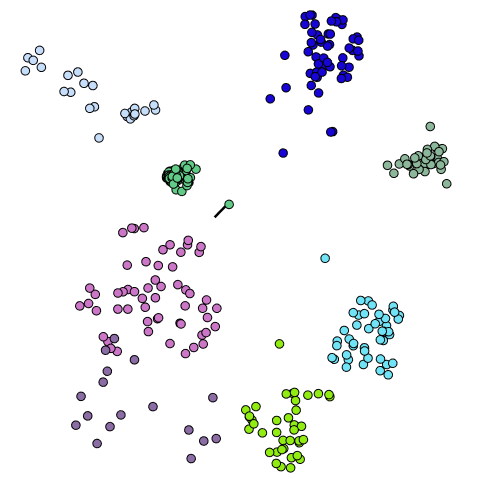
\includegraphics[width=0.8\linewidth]{pastas.png}
	\caption[Embedding of ingredients in pasta recipes]{Embedding of ingredients in pasta recipes}
	\label{fig:P2compileP0-1}
  \end{figure}

  \begin{figure}[h!]
	\centering
	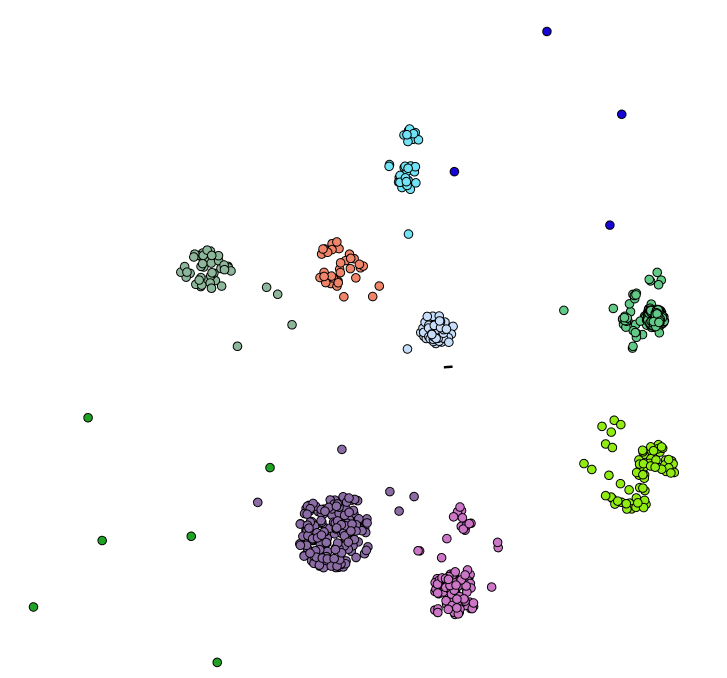
\includegraphics[width=0.8\linewidth]{salads.png}
	\caption[Embedding of ingredients in salad recipes]{Embedding of ingredients in salad recipes}
	\label{fig:P2compileP0-1}
  \end{figure}

\section{Recipe Generation}
This section mostly describes where I am currently at and problems I am encountering.

Autoencoders \cite{Makhzani16} and Generative Adversarial Nets (GAN) \cite{Goodfellow14} are well known for their capabilities
to algorithmically generate data. These are both neural network infrastructures used to produce
novel features in some vector space.

GAN work by using two components - a discriminator and
a generator. The generator takes in some random noise and outputs some data. The discriminator
is a binary classifier that determines if the input is real or generated. Both networks start
untrained and the discriminator is shown some examples of real data and gradient descent is
applied to update the weights. Then it is given a batch of the generated data and its weights
are updated again. The weights for the generator are updated based on the output of discriminator.
This provides a game mechanism where the two networks attempt to outperform one another.

An autoencoder is an encoder-decoder infrastructure that attempts to perform dimensionality
reduction in the encoder and reconstruct the input in the decoder. It's loss is calculated
during training based on how far off the output is from the input. This is an appealing design
for my application because the encoder and decoder components can be interchanged. As an example,
I could train an autoencoder on my dataset filtered by southeast Asian cuisine and train another
on southwestern US cuisine and attempt to put a southeast Asain spin on a radically different
cuisine. The other advantage with this infrastructure is that it is quite simple and easy to
implement and tune hyperparameters.

The primary issue for using neural networks for data generation
is developing a quality encoding for the training set. Using the ingredient co-occurrence
column vectors as encodings for ingredients is a one hot encoding of the data. One hot encodings
do not perform well in sparse high cardinality settings such as this. To attempt dimensionality
reductions SVD was applied to the ingredient co-occurrence matrix and the first 10 eigenvectors
were preserved from the U matrix to create dense low cardinality features for each ingredient.
A popular implementation of GAN utilizes convolutional neural networks and are known as DCGAN
\cite{Radford16}.
These have been shown to work well for generation of realistic images of faces and objects.

\bibliography{IEEEabrv,/home/austen/Documents/school/research/paper/references.bib}

\end{document}
